
\documentclass[proposal]{softeng}

\usepackage{times,color}
\usepackage{hyperref, url}
\usepackage{amsmath}
\usepackage{amssymb}
\usepackage{caption}
\usepackage{booktabs}
\usepackage{subfigure}
\title{Generating Representative Artificial Datasets for Algorithm Evaluation}
\author{\ Dan-Florin Berbec \\ \ Supervisor: Peter Bloodsworth}
\organisation{University of Oxford}
\college{Kellogg College}
\award{Software Engineering} 


 \date{November 2019}
\usepackage[parfill]{parskip}
\usepackage{amsmath}
\begin{document}

\maketitle

\newpage
\clearpage\mbox{}\clearpage

\begin{abstract}
Machine Learning algorithms become the main assets for many IT companies and their correctness is fundamental in many fields such as healthcare and finance, or simply when using an app that provides directions to a user or makes suggestions based on personal information. Computational power increases exponentially and the complexity and performance of algorithms follows the same pattern, but explainability becomes more challenging. For users, regulators, or investors that have an interest in using or investing in an AI product, the task of validating its correctness becomes difficult, especially when all that is accessible is a black box with a limited amount of test data. More importantly, AI decisions can significantly impact an end user's life and newer fields such as Deep Learning, although superior to other approaches, will be avoided in critical systems such as healthcare unless users can understand and trust the output. We aim to assess the tools and best practices currently used in XAI (eXplainable Artificial Intelligence) to reliably and independently evaluate and explain an algorithm's decision, which in turn, will provide confidence to all stakeholders that it works indeed as specified and is trustworthy for real world use cases.\end{abstract}
 
\tableofcontents
\newpage

\section{Motivation}
Algorithms are present in almost every electronic device we buy. From a simple light switch to running an OS and applications on a smartphone, their influence reaches beyond our daily decisions. For example, algorithms in a smartphone may direct a taxi driver on an alternative route based on congestion indicators set by a real-time data feed. Similarly, the prices of products in a supermarket may be influenced by low latency foreign exchange algorithms trading in an investment bank.

Another example shows the US justice system relying much more heavily on algorithms - these are used to provide a likelihood score of a convict to re-offend and is one of the main factors for a judge when deciding a sentencing\cite{jail}. The algorithm used is trained on historical data and seems to have biases correlated to a convict financial status - it may transform these biases into causations. Importantly, the underlying algorithm is private and not made available to the public for assessment.

Provided that secrecy is of utmost importance for machine learning companies across all industries, many questions arise from stakeholders: how can regulators verify the fairness/lack of bias of a financial algorithms? Will an algorithmic robot trained on worst case scenario data from the 2008 financial crises perform as well during a new financial crises with different root causes? How can a judge have confidence that no bias is part of the score given to a convict if the underlying algorithm is only accessible to a handful of people? How can investors evaluate that the product of an ML company does indeed what is says it does? 

More importantly, given the coronavirus outbreak that started in December 2019, can a doctor trust ad-hoc built AI systems that claim to diagnose the virus or help find a cure? Many companies are racing to produce products that have eye-catching accuracy and performance, but more discussion is needed on how these algorithms perform on real test data. 

For example, Darwin AI \cite{DarwinAI} claims to work on a novel Covid-19 test that uses a classification system based on CT scans to detect the spread of the virus in the lungs vs common pneumonia or healthy patients\cite{covid-net}. The authors do warn that their algorithm should not be used in production systems as it is only trained on a limited number of samples for positive patients - in an online presentation the authors describe how they initially produced a model with perfect predictions for all classes, but the determinant feature for classification was the colour of the bed the patient was lying on while the CT scan was performed. Such a model with perfect scores would have disastrous consequences if performance was the only important metric. However, similar products are already used in hospitals\cite{aids-doctors} and within the scientific community many such approaches are discussed with a focus only on performance.\cite{ai-covid-19}.

Another example within healthcare of a neural network that performs well but picks biases is described by Rich Caruana, a principal Microsoft researcher. He built a network which classifies severe cases of pneumonia vs mild ones\cite{rich-caruana}. On close inspections he notices that having asthma lowers the risk of having severe pneumonia (among several other biases). This correlation is simply explained by the extra care taken for such patients - they are more likely to see a doctor immediately if they don't feel well. If his network would be deployed to decide on real cases, it would implicitly classify them as a lower risk based on such correlations and could have catastrophic consequences - patients with asthma would likely not be admitted to hospital. Importantly, he stresses out how hard it is to detect such biases and why at least in healthcare it is crucial that a doctor understands why a classification has been made. 

Furthermore, machine learning classifiers are becoming increasingly complex: specifically, deep learning neural networks may outperform other classifiers such as SVMs or decision trees but the results are hardly explainable due to the hidden layers that aim to mimic biological brain activity. For example, an architecture for convolutional neural networks such as ResNet\cite{res-net} used for image classification can use 152 layers. It may output a superior performance compared to other architectures, but how can we detect biases and explain how it learned them, thus helping us to improve the algorithm?  Fernandez\cite{fernandez-dark-ai} describes this problem as \textit{"the ‘black box’ problem that plagues AI — our inability to peek inside exotic neural networks and understand how they work — represents one of the most urgent moral and business imperatives of our time"}.

The new general data protection regulations (GDPR) which came into effect in the European Union, further stress the importance of being able to explain automated decisions to individuals. This allows individuals to challenge decisions \cite{GoodmanB2017EUro, gdpr} and requests explanations.

Therefore, more discussion is needed on why an algorithm outputs a specific classification and how it will generalize on real data outside it's training set. This need constitutes the core motivation for this project. The aim is to survey available tools that help explain machine learning algorithms. A complete survey of such tools for every machine learning algorithm would be outside the scope. Deep Learning is a relatively new field and that neural networks become ubiquitous, a more narrowed scope is to mainly assess tools used to explain artificial and convolutional neural networks. However, many tools and techniques treat AI models as a blackbox and do not require an understanding of the underlying architecture. As such, some of these tools are applicable to a wide range of models.

Although some techniques for explainability are fairly recently developed, the interest within the scientific community in this topic is very high and many pros and cons have been discussed. The aim of this project will be two-fold: one one side we aim to discuss and compare the various techniques and on the other to survey the actual applicability in the real world, the latter not being researched as much. 

For this purpose, the project will start with some exploratory work, with implementation of neural networks and discussing approaches for explaining their outputs. The next part of the project is to work on a couple of real case studies and answer questions such as: How do commercial companies use these tools? What are the best practices used to develop trustworthy models? What features would data scientists like to see in these tools in the future to help them better understand and improve their models? Can their models be assessed independently?

This approach differs slightly form the one described in the original project proposal. Instead of evaluating the performance and determine the real value of commercial algorithms, we focus instead on explaining their decisions. This new approach is motivated after extensive reading and discussions with researchers who work with commercial companies. Aiming to challenge their IP and requesting their help in providing their data, algorithms, benchmark tools and most importantly their time, would be unrealistic and provide little value. Likely companies would dismiss such requests and furthermore it would be unlikely to outperform real employees who have a vast amount of experience in machine learning. 

On the other hand, understanding the practices used commercially to explain models, could benefit them in return by providing recommendations of how such practices can be further improved. In addition, only access to a blackbox algorithm with a few test samples would be enough to perform an attainability evaluation as opposed to entire datasets required to build the algorithm completely. It is reasonable to expect a higher willingness from private companies to collaborate under such circumstances of mutual benefit. 

\section{Introduction}


\subsection{Explainability - Problem Outline}
While simple algorithms have been around for many years aiding our decisions, complex ones now become ubiquitous in our decision-making process, many times with a significant outcome. Almost all industries including finance and healthcare or governmental institutions use algorithms to process large amounts of data to optimise spending resources. For example, a review\cite{algassessment} from the New Zealand government shows how crucial algorithms are in ensuring the wellbeing of the population. Ministries of justice, education and healthcare, customs and police, all use algorithms and data to improve their efficiency. Algorithms allow for data to be gathered and analysed, identifying key areas where young people need support or helping to aggregate data and address risks at border control. Passport and visa applications can also be automated to reduce waiting times and allow staff to manually process the ones that reach a risk threshold. However, the review clearly states that significant decisions are still currently made by humans. 

Finance also relies heavily on automation and algorithmic trading is rising very fast. Robot advisors are slowly replacing or at least aiding financial advisors to reduce the commissions charged as well as improve the performance of a fund\cite{robot}. For most financial institutions, especially large investment banks, regulators require backtesting to be executed and results sent for analysis\cite{backtesting}. This aims to ensure that trading strategies performing live today can also handle data in extreme environments such as the financial crisis in 2008.

While most of the algorithms used in decision making are currently crunching data to produce a deterministic output, newer types of algorithms within Machine Learning (ML) and Artificial Intelligence (AI) aim to train on historical data to find patterns that are applicable on new test data. From systems that recommend similar items to online shoppers to a virtual Go player that can beat a world champion\cite{alphago}, ML algorithms become increasingly trusted to take decisions that may significantly influence people's life. Huge investments are poured into self driving cars and a large number of big tech companies as well as many start ups\cite{autonomous} claim a share of this funding. These smart algorithms powering the cars may be expected to take the right decisions in noisy environments that have not been part of the training data, or ethical ones with no clear solutions, such as the trolley problem\cite{trolley}. As they are designed by humans, biases are also likely to influence the algorithm design. For such critical systems, especially where different decisions can be regarded as optimal, explainability becomes crucial, otherwise the adoption of this models will be avoided regardless of their performance. Fig \ref{fig:purposes_of_explainability} details reasons for stakeholder and the motivation for explainable AI (XAI).

\begin{figure}[h!]
\centering
  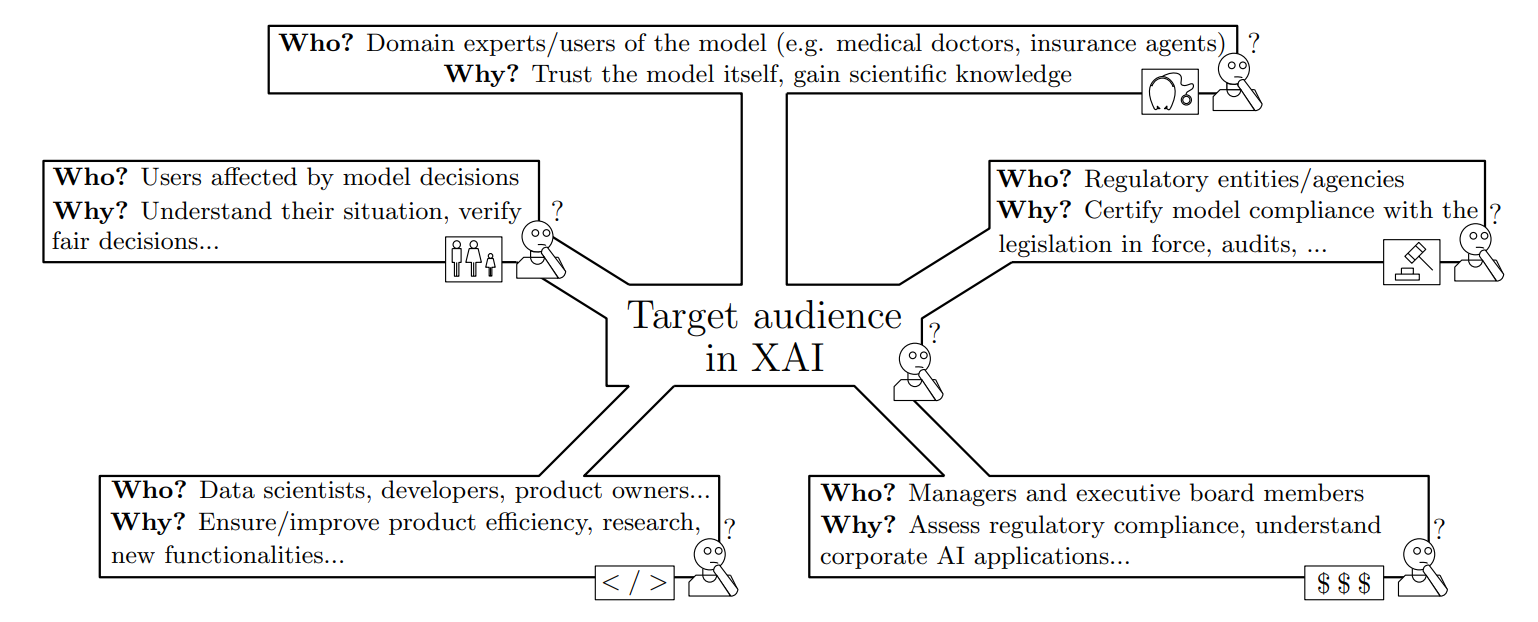
\includegraphics[width=.9\textwidth]{images/purposes_of_explainability.png}
  \caption{Purposes Of Explainability Source:\cite{BarredoArrietaAlejandro2020EAIX}}
  \label{fig:purposes_of_explainability}
\end{figure}

But the main assets of ML companies lie in developing such algorithms and preserving their secrecy. For big tech giants, such as Google, Uber or Waymo, theft of trade secrets is a serious concern and lawsuits are commonplace\cite{stealuber,waymo}. Algorithmic trade secrets, such as trading software, are also crucial in the financial industry, and any attempt for industrial espionage is thoroughly chased\cite{jeopardy}.

Therefore, most of the time, a blackbox is provided to an external audit or potential investor with limited test data. Furthermore, this data could easily be proprietary as well and cleaned to fit the claims of the product. Currently, it seems that stakeholders do not have any means to independently verify that an algorithm does indeed what it says it does. 

With the increasing rise of tech startups, we may assume that in the near future, multi billion dollar companies may have only a handful of employees with a codebase living in the cloud and their main asset being IP. Their algorithms may have significant decisions for the public, yet understanding why a decision has been taken may be challenging to explain. In particular, end users should always be able to understand exactly what factors mattered when an automated decision is taken (e.g. Why has my loan been denied? Why was I not admitted to the hospital when ill? Where did my pension's trading strategy go wrong?) - importantly such explanations should also be easily understandable. From a human computer interaction perspective this will help users accept decision more easily: a good example is Netflix, which provides clear explanations to users for new shows it recommends based on previous viewings. 

\subsection{Proposed work}

The aim of this project is to investigate the available tools used by researchers and other stakeholders in understanding how their models behave when making classifications. Ideally, the main focus will be to compare tools and processes that can fit scenarios where the model is treated as a blackbox with a limited amount of test data. The next stage is to assess the suitability of these tools within real case studies and eventually make realistic proposals for improvements. The focus will be on explaining artificial and convolutional neural networks, but the general guidelines derived should be applicable to any organisation independent of the size, technology stack or industry.

Deep learning mainly provides two types of algorithms: supervised and unsupervised learning. Supervised learning is used for classification purposes while unsupervised learning aims to find patterns within a data sets that are not mapped to specific labels.

Artificial neural networks (ANN) are trained on test data sets and make predictions on new inputs. Their efficiency can usually be measured on how accurate their predictions are. For example, given a dataset of customers leaving a bank, a ANN can make future predictions based on independent variables on whether a customer is likely or not to leave the bank as well. An ANN could also decide based on income and age, whether a customer should be granted a loan or not. Another example could be a ANN making stock price predictions. While the algorithm is not public, it would be crucial for customers to have the ability to understand its behaviour before placing any money of their savings.

The aim is also to test the behaviour of the algorithm under worst case scenarios or perform other modifications to the dataset to identify potential poor performance that impacts the validity of testing and in particular pick any unhealthy biases. The project will evaluate a number of open source ANNs used in a variety of fields such as healthcare, finance, or law. The algorithms may be packaged as runnable code with training and test data or as a black box with test data only. 

A first step is to review the historical and current approaches used to train and explain model predictions. By reviewing the current literature, the most suitable tools and techniques will be selected. The next stage will be to briefly discuss the architecture or neural networks and provide an implementation for an artificial and convolutional network. The solutions identified in the background literature can be applied and their performance can be assessed. Are these solutions indeed able to explain how the models make predictions and identify biases? What are the computational requirements and how feasible are they if they were used in real world scenarios?

The second step will discuss specific use cases. Of particular interest are models that perform within healthcare, especially during the coronavirus pandemic where AI is heavily relied on to diagnose or find treatments. Many solutions are rapidly deployed and their correctness can be crucial in reducing the number of deaths caused by COVID-19. Informal discussions with software engineers designing these models will be conducted aiming to find out what tools and best practices are used to ensure correctness of deployed models. Where possible, the selection of models discussed in the background literature will be applied on such models to make further inferences. This will of course be done with the express consent of the companies or where such models are open source.

The expected outcome will present the reader with a set of best practices and tools currently used in academia and in the real world for explaining AI models. A comparison of the tools and use cases they cover best and what is needed in the future will be addressed. These examples do not aim to provide a silver bullet for implementing foolproof explainable models, but rather a sample of what might be useful in the development and testing process of new models to ensure that correct outputs are produced for the right reasons. This is subject to further background literature and the rapid growth of new ideas being published in the field.

Further notes:
novelty of exaplinability -whhy and what that means. models are designed and trained to perform well and reduce the loss function not to be explainable to humans in an intitive way

] J. Angwin, J. Larson, S. Mattu, and L. Kirchner, “Machine bias,”
https://www.propublica.org/article/machine-bias-risk-assessments-in-criminal-sentencing
[Accessed May 24, 2019], 2016

http://opendatascience.com/ai-black-box-horror-stories-when-transparency-was-needed-more-than-ever/
-not everything need to be explained

\newpage
\section{Background Literature}
\subsection{Overview}
This chapter explores the current landscape of solutions available. Only a handful of papers researched are older than five years, yet the amount of publications available within this time-frame is surprisingly much higher than estimated at the start of this project and new research is published at a lightning speed as shown in figure \ref{fig:evolution_publications}. This is no doubt a good sign suggesting that research community and commercial developers are indeed taking a step back to ensure that models produced can be trusted. However, the topic of explainability still needs significantly more time to reach maturity: there are no processes or clean patterns that fit most problems. It is also worth noting that many talks and blogs discuss machine learning related topics and while some of them are of questionable value, others have great insights written by experts in this area and worth to be included in this chapter, with a clear priority however for peer reviewed articles.

\begin{figure}[h!]
\centering
  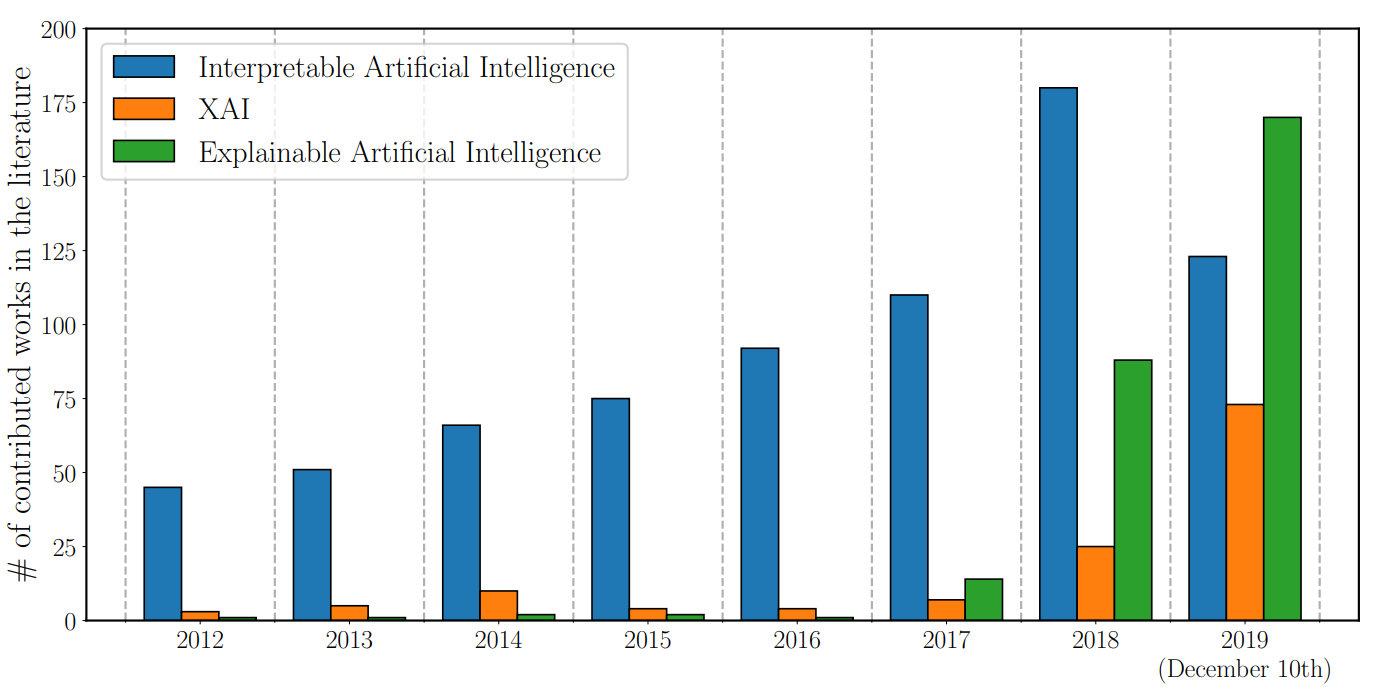
\includegraphics[scale=0.5]{images/evolution_publications.png}
  \caption{\textit{"Evolution of the number of total publications whose title, abstract and/or keywords refer to the field of XAI during the last years. Data retrieved from Scopus (December 10th, 2019)"} Source image and text:\cite{BarredoArrietaAlejandro2020EAIX}}
  \label{fig:evolution_publications}
\end{figure}


As we are interested mainly in Deep Learning models, we will start with a brief introduction to artificial and convolutional neural networks. The next step will be to contain the vague definition of explainability/interpretability. What does "explainable" mean and what metrics are used to measure it? We then move on to provide an overview of the current approaches at an abstract level: do tools/methods need access to the structure of the model or can they treat it as a balckbox? What precesses are available to extract logic from the model and what tools are ready for use now with moderate resources?

We then move to a more in depth discussion with pros and cons of some of these tools that have the best potential to evaluate models. A subsection will also be dedicated to research about strategies that compare them with one another. What strategies can be used to asses the correctness of interpretability methods themselves? Finally we narrow down to a selection that can be used in the next chapter and further applied to commercial models. 

This is by no means an exhaustive overview of tools, such an approach would be well beyond the scope of this project. Neither is the intention to implement new approaches from scratch: it would be challenging to get this right and of little value for the purpose of this project.

\subsection{What is explainability?}
Explainability is a new filed in AI (XAI - eXplainable AI) and the focus is mainly to explain what features in the input significantly influence the model to provide a higher probability to a class than to others. Arrieta, Alejandro Barredo et al.\cite{BarredoArrietaAlejandro2020EAIX} define XAI as: \textit{"Given an audience, an explainable Artificial Intelligence is one that produces details or reasons to make its functioning clear or easy to understand"}  But what can we classify as a well explained decision? What metrics can be used?

In the book Interpretable Machine Learning, Christoper Molnar \cite{molnar2019} identifies several attributes of what makes a useful explanation and we summarise key aspects of these: for example, fidelity relates to "how well the explanation approximates the prediction of the black box model". This is crucial in determining how suitable the technique of extracting the explanation is. If fidelity is low, the explanation should simply not be used.

Consistency relates to differences in explanations provided among the same inputs across different models (e.g. logistic regression vs a deep neural networks). In other words, if you have two doctors with different specialities, they could both conclude the same diagnostic but for very different reasons. In such cases, the explanations should be different, but should be similar when the deciding factors are indeed the same.

Stability is similar to consistency but evaluates explanations across different inputs within the same model. When inputs have similar features with only slight variations, the explanations should also be similar. Otherwise, it would be hard to understand the underlying behaviour of the model or whether explanations are indeed relevant, except of course for rare cases where such small differences are indeed expected to significantly influence the outcome.

Molnar identifies comprehensibility as being the "elephant in the room". Explanations need to be understandable and this depends directly on the type of users and the size and complexity of the explanation. Based on these explanations, users should in turn be able to replicate the model behaviour. This attribute is directly linked to representativeness: does the explanation refer to individual instances or to the internal structure of the algorithm. Individual instance explanations are useful for a general idea of the behaviour but detailing the inner working of what features a specific class is dependent on together with the logic behind it can be more useful.

R. Guidotti et al. \cite{guidotti} define interpretability as \textit{"an “interface” between humans and a decision maker that is at the same time both an accurate proxy of the decision maker and comprehensible to humans"}. Further to accuracy and fidelity, this paper defines further characteristics: it puts a strong empahsis on global vs. local interpretability. If the logic of the model can be deduced to predict any possible outcome, the model is \textit{completely interpretable}, in contrast to reasoning about one single input. 

Interestingly, explanations may also need to have time limitations based on how urgent a further action from the user is needed. Thus, explanations should grow from simple and precise to complex ones depending on the requirements. This is directly related to the domain knowledge of the user.

This shows that no gold standard can be applied to explain any type of models. While these are general guidelines, different types of models and requirement may put an emphasis on all or just a selection of these depending on the specific goals of the model. For example, we may sometimes want to explain only local inputs but other times a thorough understanding of the structure can be required (e.g. a financial audit in an investment bank for a risk team). 

Arrieta, Alejandro Barredo et al\cite{BarredoArrietaAlejandro2020EAIX} propose a direct mapping between the goals achieved by explanations and the target audience, some of which we mention and discuss here:

Trustworthiness is the main goal of XAI but is of particular importance for domain experts and end users - they would be unliekly to use a model if they don't trust it. Another goal is causality - this can be of interest primarily to regulators and domain experts. While a model only learns correlations, these should be inferred as causal relationships only when aggregated with vast domain knowledge. Importantly, causality should not be implied by correlations as this could easily lead to unfair biases. This would be related to another goal: fairness. This ensures \textit{a clear visualization of the relations affecting a result...[and] should be considered as a bridge to avoid the unfair or unethical use of algorithm’s outputs}. A further indirect goal is represented by privacy awareness: explainability can ensure that data captured inside the structure of a model is not breaching privacy. Furthermore, the authors also identify types of explanations: these can be either text based, visual or based on examples.

Gilpin, Leilani H. et al.\cite{GilpinLeilaniH} also mention completness as a main goal for explanations:\textit{it must produce descriptions that are simple enough for a person to understand using a vocabulary that is meaningful to the user}. They suggest there is a clear tradoff between accuracy of explanations and completeness, in that complex explanations become hard to interpret, and in turn, simple explanations will not provide predictive skills to a human to mimic the model - which is importnat for making the model trustworthy. Another interesting observation from this paper is the risk that arises from an ethics perspective: an accent may be put on making explanations perusaive instead of fair which poses further questions about the role of human factors and ethics that may become challanges in the future.

\subsection{Current approaches towards XAI}
Ideally, explainability should be incorporated by design and should start at the very beginning when exploratory data analysis is performed. 

Khaleghi \cite{khaleghi} explains the importance of identifying shortcoming of the training data such as class imbalance issues or dealing with missing data. This can be achieved by using different types of charts to plot the data and using statistical analysis to fill in missing values. Importantly, features should also be explainable and meaningful to the end user who should also intuitively asses their importance. When the number of features in a dataset is too large, dimensionality reduction techniques such as principal component analysis can be applied.

At a model implementation stage, two braod categories of models can be identified: the ones that have an inherently interpretable structure such as decision trees, and those that are significantly more complex such as SVM or neural networks, and even with access to code, their predictions cannot be immediately inferred. Yang et al. (2019) \cite{YangFan2019EEWG} divide these two categories into ML (machine learning) and IML (interpretable machine learning) as shown in figure \ref{fig:iml}. 

\begin{figure}[h!]
\centering
  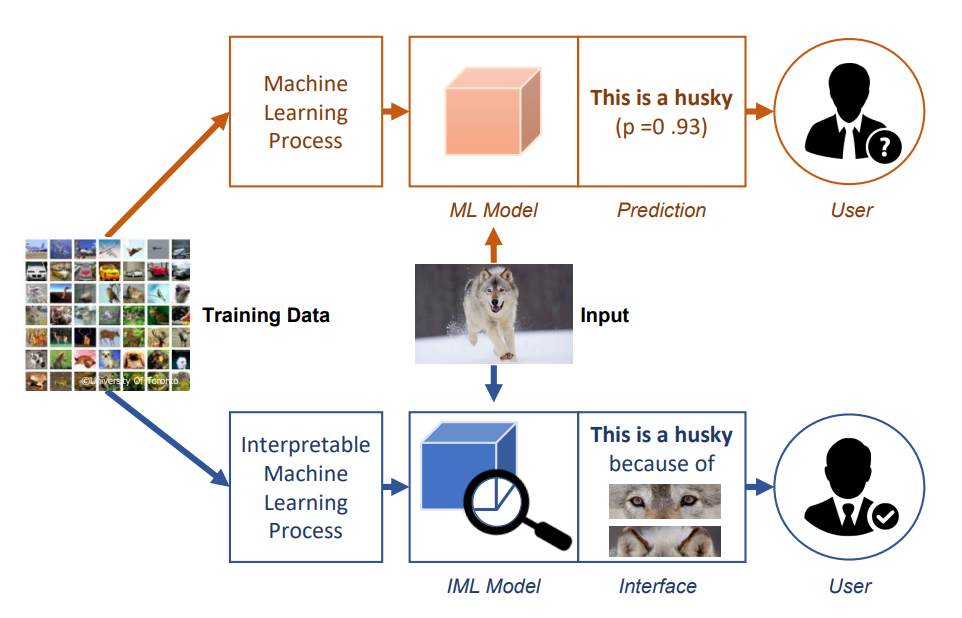
\includegraphics[width=.8\textwidth]{images/iml.png}
  \caption{ML only provides a probability score for its classification while IML explains the decision taken. The use is satisfied when a clear explanation is provided rather than a high probability Source of image:\cite{YangFan2019EEWG}}
  \label{fig:iml}
\end{figure}

One of the classic interpretable models is logistic regression that can perform binary classification assuming the inputs and predictions are linearly dependent. Such models can be easily plotted on a graph for visualisation and are inherently easy to understand. Another example are decision trees: they are used by humans in every day tasks and their output is simple to understand or reproduce - as long as such trees don't grow above our ability to visualise them (e.g. random forests are composed of hundreds of trees and are not interpretable). Other explainable models incdlude K-Nearest Neighbours or rule based learners, both models able to provide explanations thorugh their inherent structure. Probabilistic models using Bayes' theorem are more complex, but powerful and understandable by domain experts especially when the probability for an event to occur is strictly dependent on other prior conditions. For example, in computational neuroscience, The Bayesian brain hypothesis is extensively used to explain different parts of the brain at an abstract level \cite{YairWeiss2002Miao}.

Even in deep learning many new architectures emerge that incorporate explainability by design, in particular for neural networks which have a significantly harder to explain structure compared to other classifiers. For example, Alvarez-Melis et al (2018)\cite{alvarezmelis2018robust} propose Self-Explaining Neural Networks which work by \textit{"progressively generalizing linear classifiers to complex yet architecturally explicit models"}. Such designs aim to make explanation understandable, faithful and consistent. Similarly, Al-Shedivat et al(2017)\cite{alshedivat2017contextual} propose Contextual Explanation Networks: these \textit{"generate parameters for intermediate graphical models which are further used for prediction and play the role of explanations."} These models do not offer a clear understandable interpretation and more research is needed to develop them further before they can be used commercially. They also can't be applied to existing models. However, there will be classic choices of models that are inherently transparent as long as the complexity is low. 

We learn that the choice of a good model that is both interpretable and provides a high performance is challenging: high performance models will encapsulate a large degree of complexity, thus reducing interpretability. Even models described as inherently explainable will become opaque depending on the number of features and the number of layers in their structure, simply because human factors such as short term memory are limited.

For black box models such as neural networks, explainability is mainly assessed after the model has been created, mostly with model agnostic techniques. However, this approach does allow for improved models to be generated after assessment in an iterative process and are not different than other methods used to improve performance such as hyper parameter tuning: when issues are found, they can be fixed and the model is retrained.

In a broad overview, Sheldon Fernandez \cite{fernandez-dark-ai} describes four general approaches currently used to interpret and explain blackbox models, which grew from theoretical scenarios into commercial specific use-cases, but usually as the author claims, with limited success and with exaggerated claims about the accuracy of model interpretability. The first approach is to create \textbf{perturbations} of a particular input set and asses the impact of the predicted decisions. \textbf{Backwards propagation} estimates the weight of neurons in each layer to derive an importance score for each feature. Another approach is to use a simple but more explainable model, \textbf{a proxy}, that is trained to imitate the complex one (e.g. a decision tree imitating a deep neural network). The last approach, \textbf{Activation Optimization} searches for input patterns to maximise/minimise the classification probability for an input.  

Arrieta, Alejandro Barredo et al \cite{BarredoArrietaAlejandro2020EAIX} would classify such techniques as \textit{Explanation by simplification} (same concept as using a proxy model) or \textit{Feature relevance explanation}, where the aim is \textit{to describe the functioning of an opaque model by ranking or measuring the influence}. Feature relevance can be achieved by using game theory principles. \textit{Visual explanations} can also be used along with feature relevance to derive explanations. The actual implementations of tools will be using a mix of the approaches.

Yang et al. (2019) would simply classify the explanations as either global or local and either intrinsec or posthoc. For example the proxy method is described as a posthoc global mimic learning. Figure \ref{fig:interpretation_scope} shows how a simple, inherently interpretable model, the student, mimics the output of the teacher, the deep neural network. The image also provides excellent examples for all other types of explanation combinations.

\begin{figure}[h!]
\centering
  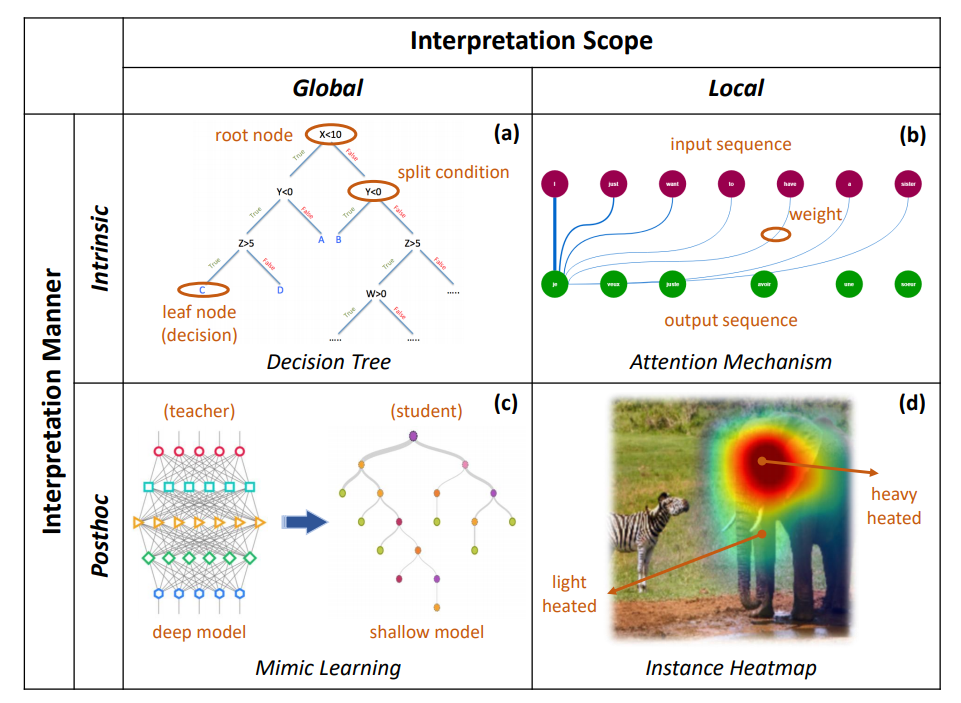
\includegraphics[width=.8\textwidth]{images/interpretation_scope.png}
  \caption{Types of interpretation manners for different scopes:\cite{YangFan2019EEWG}}
  \label{fig:interpretation_scope}
\end{figure}

Any of these techniques has benefits and limitations. In the article mentioned, Fernandez further details some limitations: for example, using a proxy to simplify a model will rather provide hints on how the underlying algorithms performs. While these may be useful, they may not be accurate and should not be relied upon in mission-critical systems. Gilpin, Leilani H. et al.\cite{GilpinLeilaniH} argue however that such models provide a \textit{"quantifiable relationship between
complexity and faithfulness"} which makes such approaches comparable with one another, although they agree that rule extraction for exmpale will likely not be a faithful representation of the model.

Other techniques will perturb the input to assess the importance of its features. Perturbing such features even slightly can produce opposing results and furthermore, they can only be applied to a number of limited inputs and would not account for global behaviour. Perturbing data with a large number of features would further also increase the computational cost exponentially.

In all cases, the scores attributed to different features will need to be interpreted by the user and models improved accordingly. Inherently, such decisions would be debatable by different users. In healthcare for example, two specialists could have different domain views on weather some features are more important than others and trusting a model would be a subjective preference.


For our purposes, we need to identify solutions that are readily available to developers, easy to implement on current models and understandable by all stakeholders, ideally applicable to any type of model and not exclusive to neural networks.




-area I am going to consider and why and area I will not consider and ww
- mostly interested in black box approaches as this allows independent evaluation
-


robustness - similarity among instances using sensitivity as the metric. Need for stable prediction model and explanation generator.


split into categories of approaches , not only what the stuff is and educate the reader.

- developers require an deep understanfing of how the models arhitecure learns so they can improve it, whil those using it need to understand how it works as a whole when a decision is taken - fro example a written text on what features are important 

Influence Functions -

%Importance scores (aka saliency heatmaps) - most common type of exmplanbation

%Anchors methods: https://homes.cs.washington.edu/~marcotcr/aaai18.pdf

%Decision trees  - https://link.springer.com/chapter/10.1007/978-3-319-46307-0_29

For our purposes, we need to find solutions that are available to developers, easy to implement on current models and understandable by all stakeholders.

The perturbation mechanism methods have two main advantages: they are typically easy to implement, and they are not limited to a specific model architecture but compuytationally expensive if the models are high dimentaional.

Gradient-weighted Class Activation Mapping (Grad-CAM)

responsible AI - fairness, model explainability and accountability at its core

difference between explainable by design and external techniques
\subsection{LIME}
what is useful, what I learn, what areas are weak, what can be improved 
like a critic, this area can be better, waht to take forward

(LIME) approach provides explanation for an instance prediction of a model,
\subsection{SHAP}
\subsection{Evaluation Strategies for XAI methods}
As seen so far, many approaches and tools have been developed in recent years, with a particular aim to explain opaque models, in particular within deep learning. One of the main goals of explanations is to satisfy the expectations of human users and gain their trust:  this makes benchmarking them against each other a challenging topic, and there are not many mature strategies for such evaluations. This is however important, especially in commercial settings, where choosing the right explainability tools for the right model, users, and requirements may simply make the difference between a fair model and one with negative consequences.


Bibal et al.(2019) \cite{bibal2019user} put an emphasis on the role of HCI in XAI. To evaluate explanations, experiments should involve users. Such users should perform simplified tasks to measure interpretability of the model. The authors propose three steps: identifying what needs to be measured - if the metrics are clearly defined, the experiment will not need a large number of participants. Secondly identifying the right user profile - participantws hould have a similar domain knowledge as real users. Third are the type of metrics used: for example \textit{measuring users’ errors, time and users’ opinions} would be a good start for such experiments. 

For example, if LIME and Shap are compared, we can measure comprehensibility by simply asking participants which explanations are clearer - time and users' opinions would be suitable indirect metrics. To measure accuracy of explanations, we can ask participants to learn the models and make predictions. These classifications can be compared with the ones produced by the models.

Lage, Isaac, et al. (2019) \cite{LageIsaac2019AEot} have also published researched  that aims to identify which \textit{"properties of decision sets are most relevant for human users to be able to use the explanations for a set of synthetic tasks"}. They  measure response time as a dependency on the explanation size and the accuracy in simulation tasks.

Yang et al. (2019) \cite{YangFan2019EEWG} also review methods to evaluate explainability. A metric such as fidelity, is completely explainable by models that already offer inherent interpretations (e.g. decision trees). But for posthoc explanations, full fidelity cannot be provided. One approach they describe to measure fidelity of a proxy is to \textit{"check the prediction variation after the adversarial changes made according to the generated explanations"}. If the explanation is faithful the prediction confidence of the complex model (the teacher) on the newly perturbed input should be significantly lower. For example, if age is provided as an explanation for a specific disorder, then removing or perturbing this attribute should lower the confidence of the model when it reclassifies it. 

For CNN, the approach would mask the important areas identified in the image and a lower class probability should be provided if the explanation was indeed faithful. For this type of evaluation, robustness should also be quantified along with fidelity as models can be "fragile to adversarial perturbations" and suggest sensitivity as a good metric to measure robustness. This should ensure that predictions are stable for both the model and explanation generator.

Wong et al. (2019) \cite{LinZhongQiu2019DERD} use a very similar approach as the one described on actual explainability methods. They train a CNN with a ResNet-50 architecture and choose LIME, SHAP, Expected Gradients, and GSInquire for comparisons. Interestingly, they introduce two scores for evaluation: the impact score that measures the confidence difference between the original image and the altered image with neutral patches on the segments identified as important by the explainability method. The Impact coverage \textit{"assesses the percentage coverage of adversarially impacted factors in the input."} Their approach is opposite to HCI and described as a more \textit{"machine-centric strategy"} as no human participants are involved. Figure \ref{fig:decision_change} shows how the classification can change if the area identified as important in the explanation is covered with a patch.

\begin{figure}[h!]
\centering
  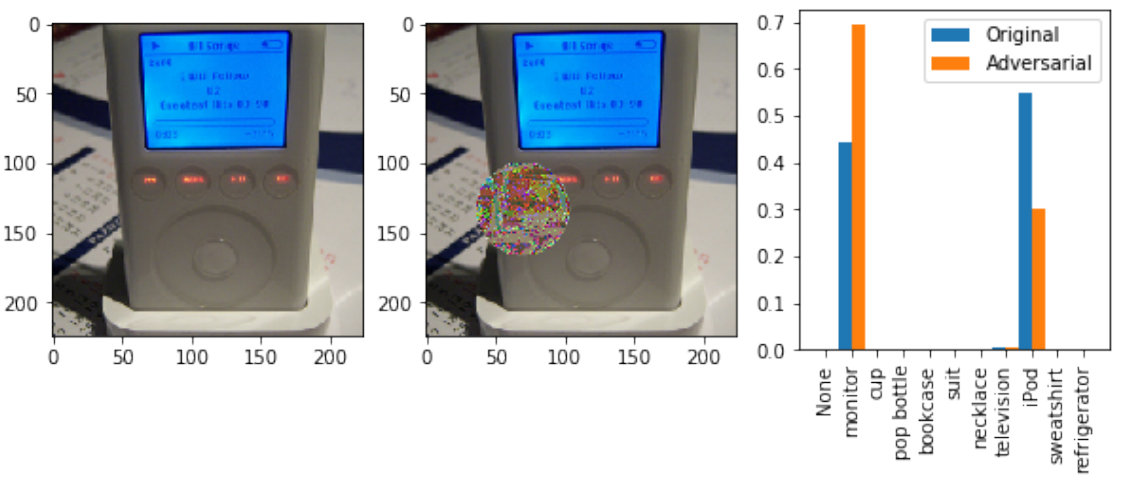
\includegraphics[width=.8\textwidth]{images/decision_change.png}
  \caption{\textit{"Example of a directed erroneous decision due to adversarially impacted area. (left) original
untampered image, (center) tampered image with an adversarial patch, (right) prediction confidences
of decisions made with untampered image and adversarially tampered image. The adversarial patch
led to a change in decision."}: Image and text source: \cite{LinZhongQiu2019DERD}}
  \label{fig:decision_change}
\end{figure}

As a critique, the algorithm that scores highest is developed commercially by the authors of the papers, and thus these scores will not be discussed further, yet the practical and quantifiable approach described is one of the first published within XAI.


\subsection{Selection of methods - reflection on why these are best to be compared}
 We do not aim to implement techniques from scratch based on papers

\subsection{Artificial Neural Networks}

Artificial Neural Networks have become very popular in recent years for creating Artificial Intelligence algorithms. The aim is to teach a machine how to extract and learn features of a data set to make new predictions by replicating processes happening in the biological brain. Using a simplified neural representation: the dendrites, nucleus and axon of a neuron are respectively abstracted for a theoretical algorithm as the input, processing node, and output. This idea dates back from 1957 when Frank Rosenblatt demonstrated the first perception: "the first machine which is capable of having an original idea" \cite{rosenblatt}, but only recently has computational  power increased to develop the ability to make predictions.

The ANN is built using visible input nodes (data you can see - ex. age, address, education, job status) that feed into several hidden layers of neural nodes further feeding into output nodes, the visible binary or categorical output, for example a loan application being granted or declined. A node in any layer can be connected to one or many  nodes in the next layer. Due to the complexity of the connections in the middle layers and the fact that the data is not easily readable, the middle layers are called hidden layers (fig \ref{fig:simplenetwork}).

\begin{figure}[h!]
\centering
  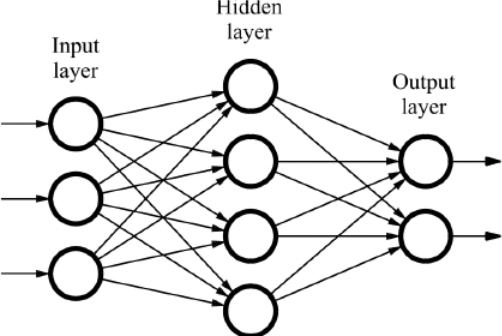
\includegraphics[scale=0.4]{images/simple-neural-network.jpg}
  \caption{Simple neural network with one hidden layer \cite{simpleneural}}
  \label{fig:simplenetwork}
\end{figure}

Each neuron in the network receives input from other nodes and computes this into a single output that feeds into other neurons or output nodes. A simple approach for a neuron's prediction could be to multiply an adjustable weight to each incoming input. To avoid producing zero values for zero inputs a bias can be added further as shown in eq  \ref{neuron}

\begin{equation}
\label{neuron}
 \sum_{i=1}^{n} {x_{i}} {w_{i}} + {b_{i}}  
\end{equation}



When the input \( {x_{i}} {w_{i}} \) is significantly less than the bias \({b_{i}}\) this implies that input has little effect. But over the training period the weight will be adjusted accordingly to overcome the effect of the bias. The final sum is not bounded and thus can be largely different than the output of other nodes. Activation functions are used to contain this value between a specific range, most commonly between -1 and 1. For example, a simple activation function, binary step, can solve this issue. But this cutoff function however will drop many small details and may only be used in binary classification problems. While there are many activation functions available, the most commonly used alternatives are the \textit{sigmoid} function and \textit{rectified linear unit} (ReLu) which preserve and propagate more information as shown in figure \ref{activation_funtions}. 

\begin{figure}
    \centering
    \subfigure[Binary Step]
    {
        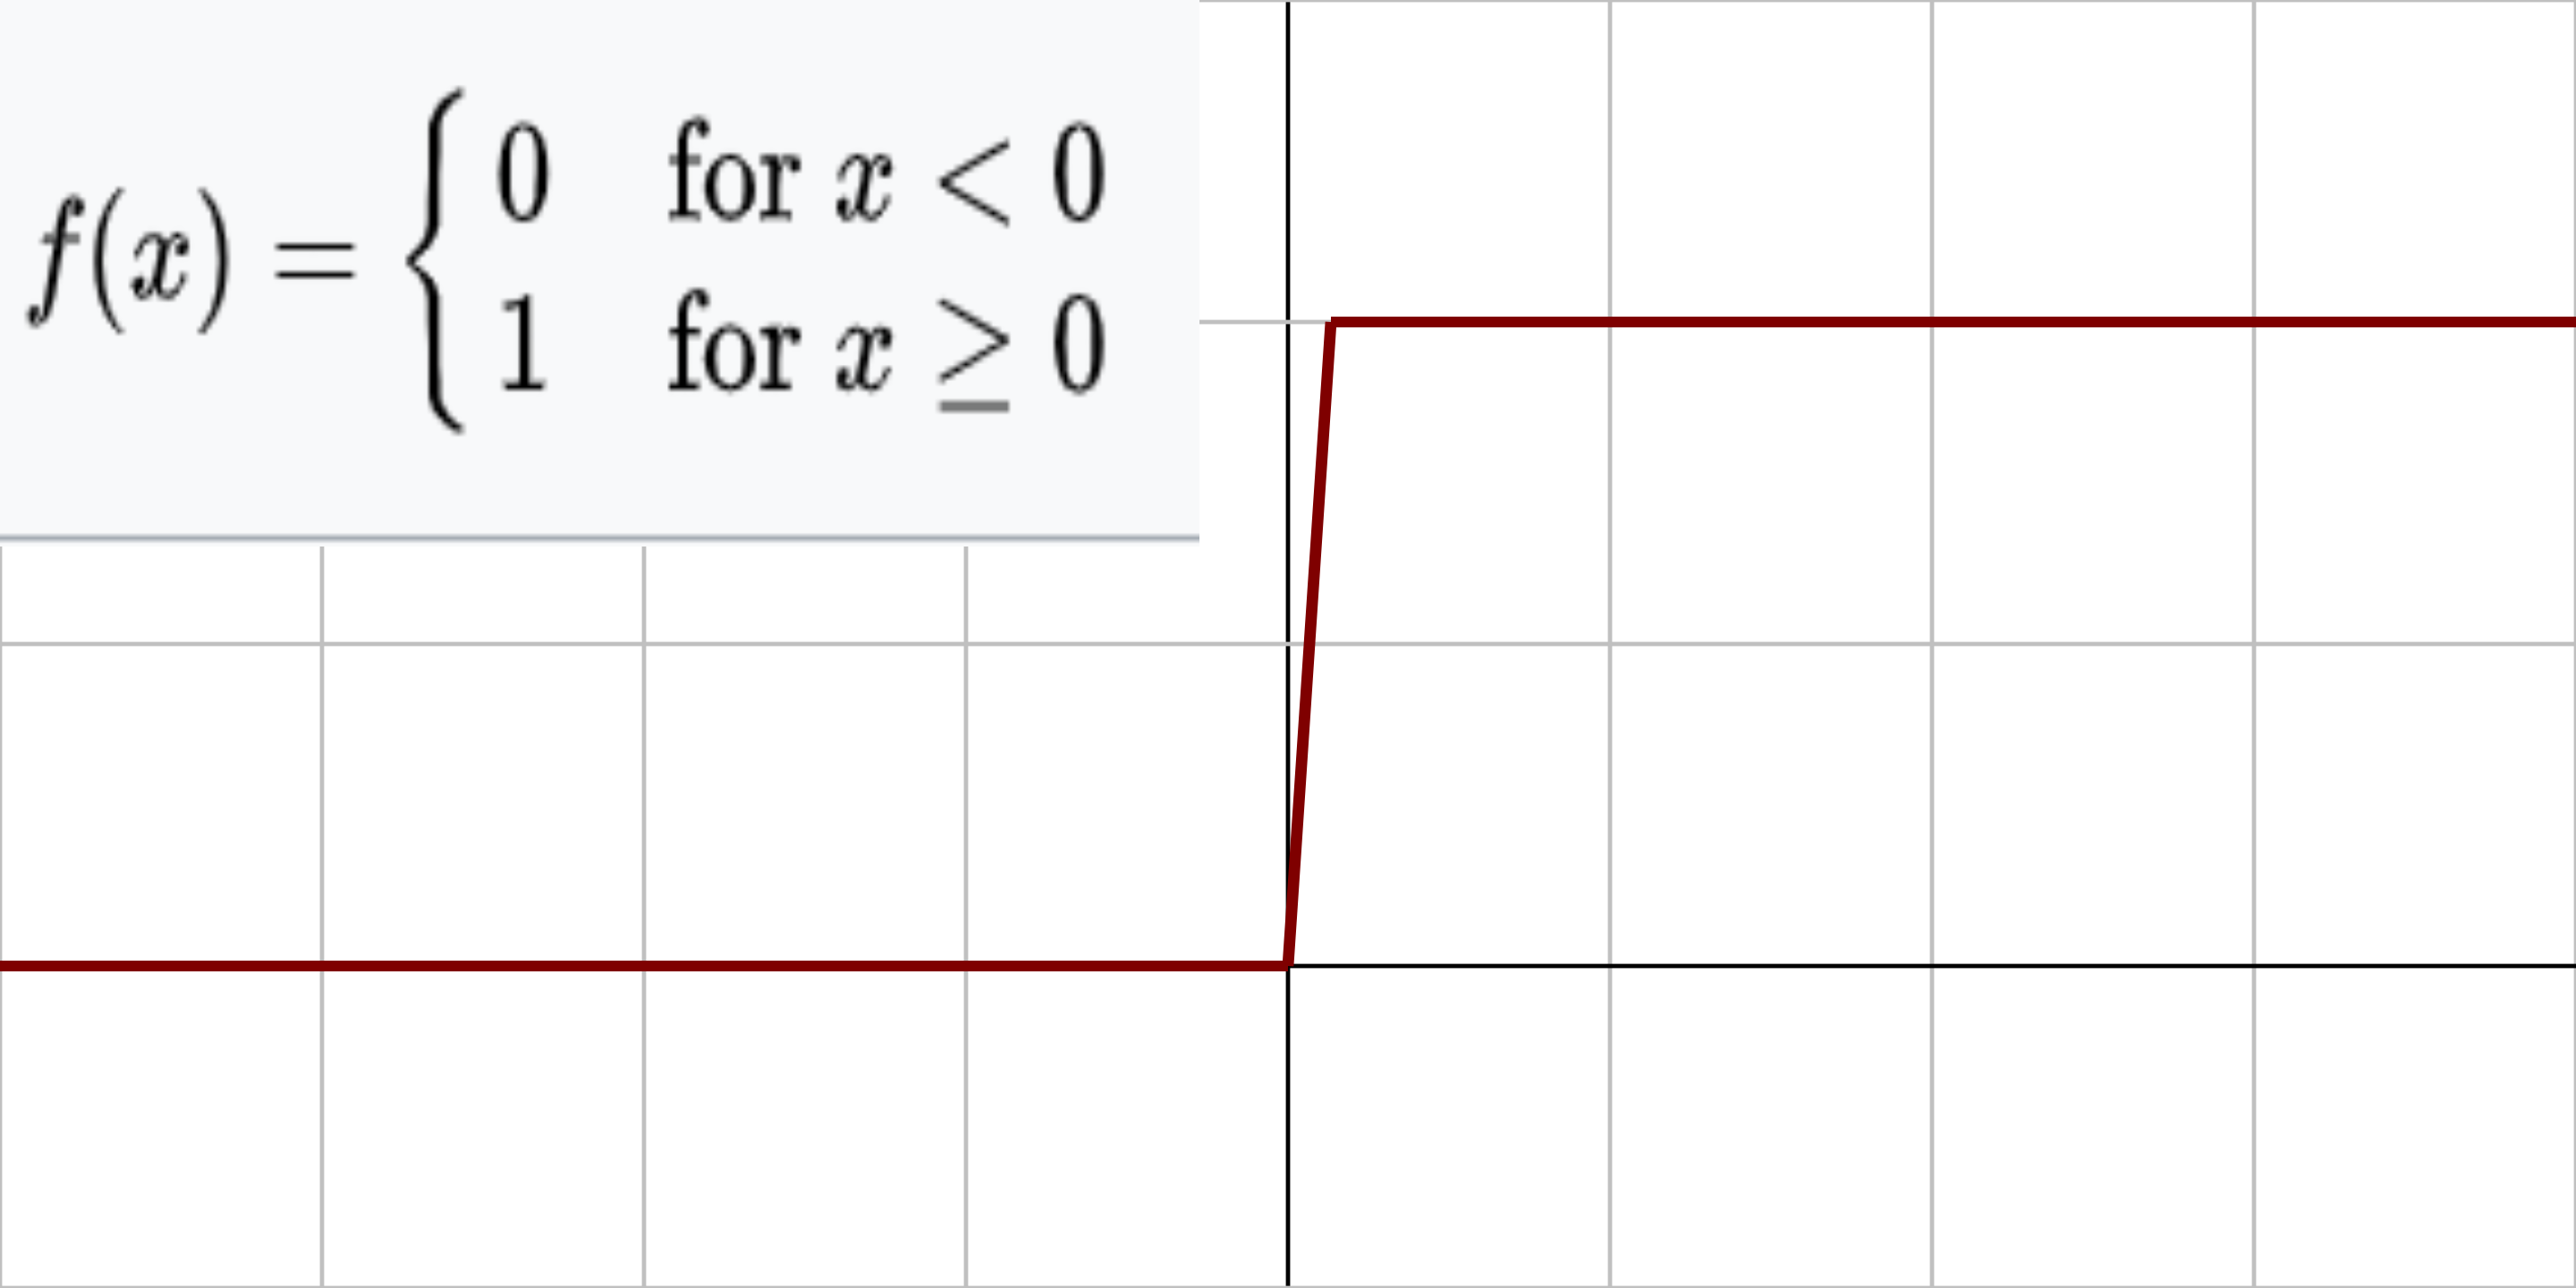
\includegraphics[width=1.8in]{images/activation_binary_step_1.png}
        \label{fig:first_sub}
    }
    % \\
    \subfigure[ReLu]
    {
        
\includegraphics[width=1.8in]{images/activation_rectified_linear.png}
        \label{fig:second_sub}
    }
    \subfigure[Sigmoid]
    {
        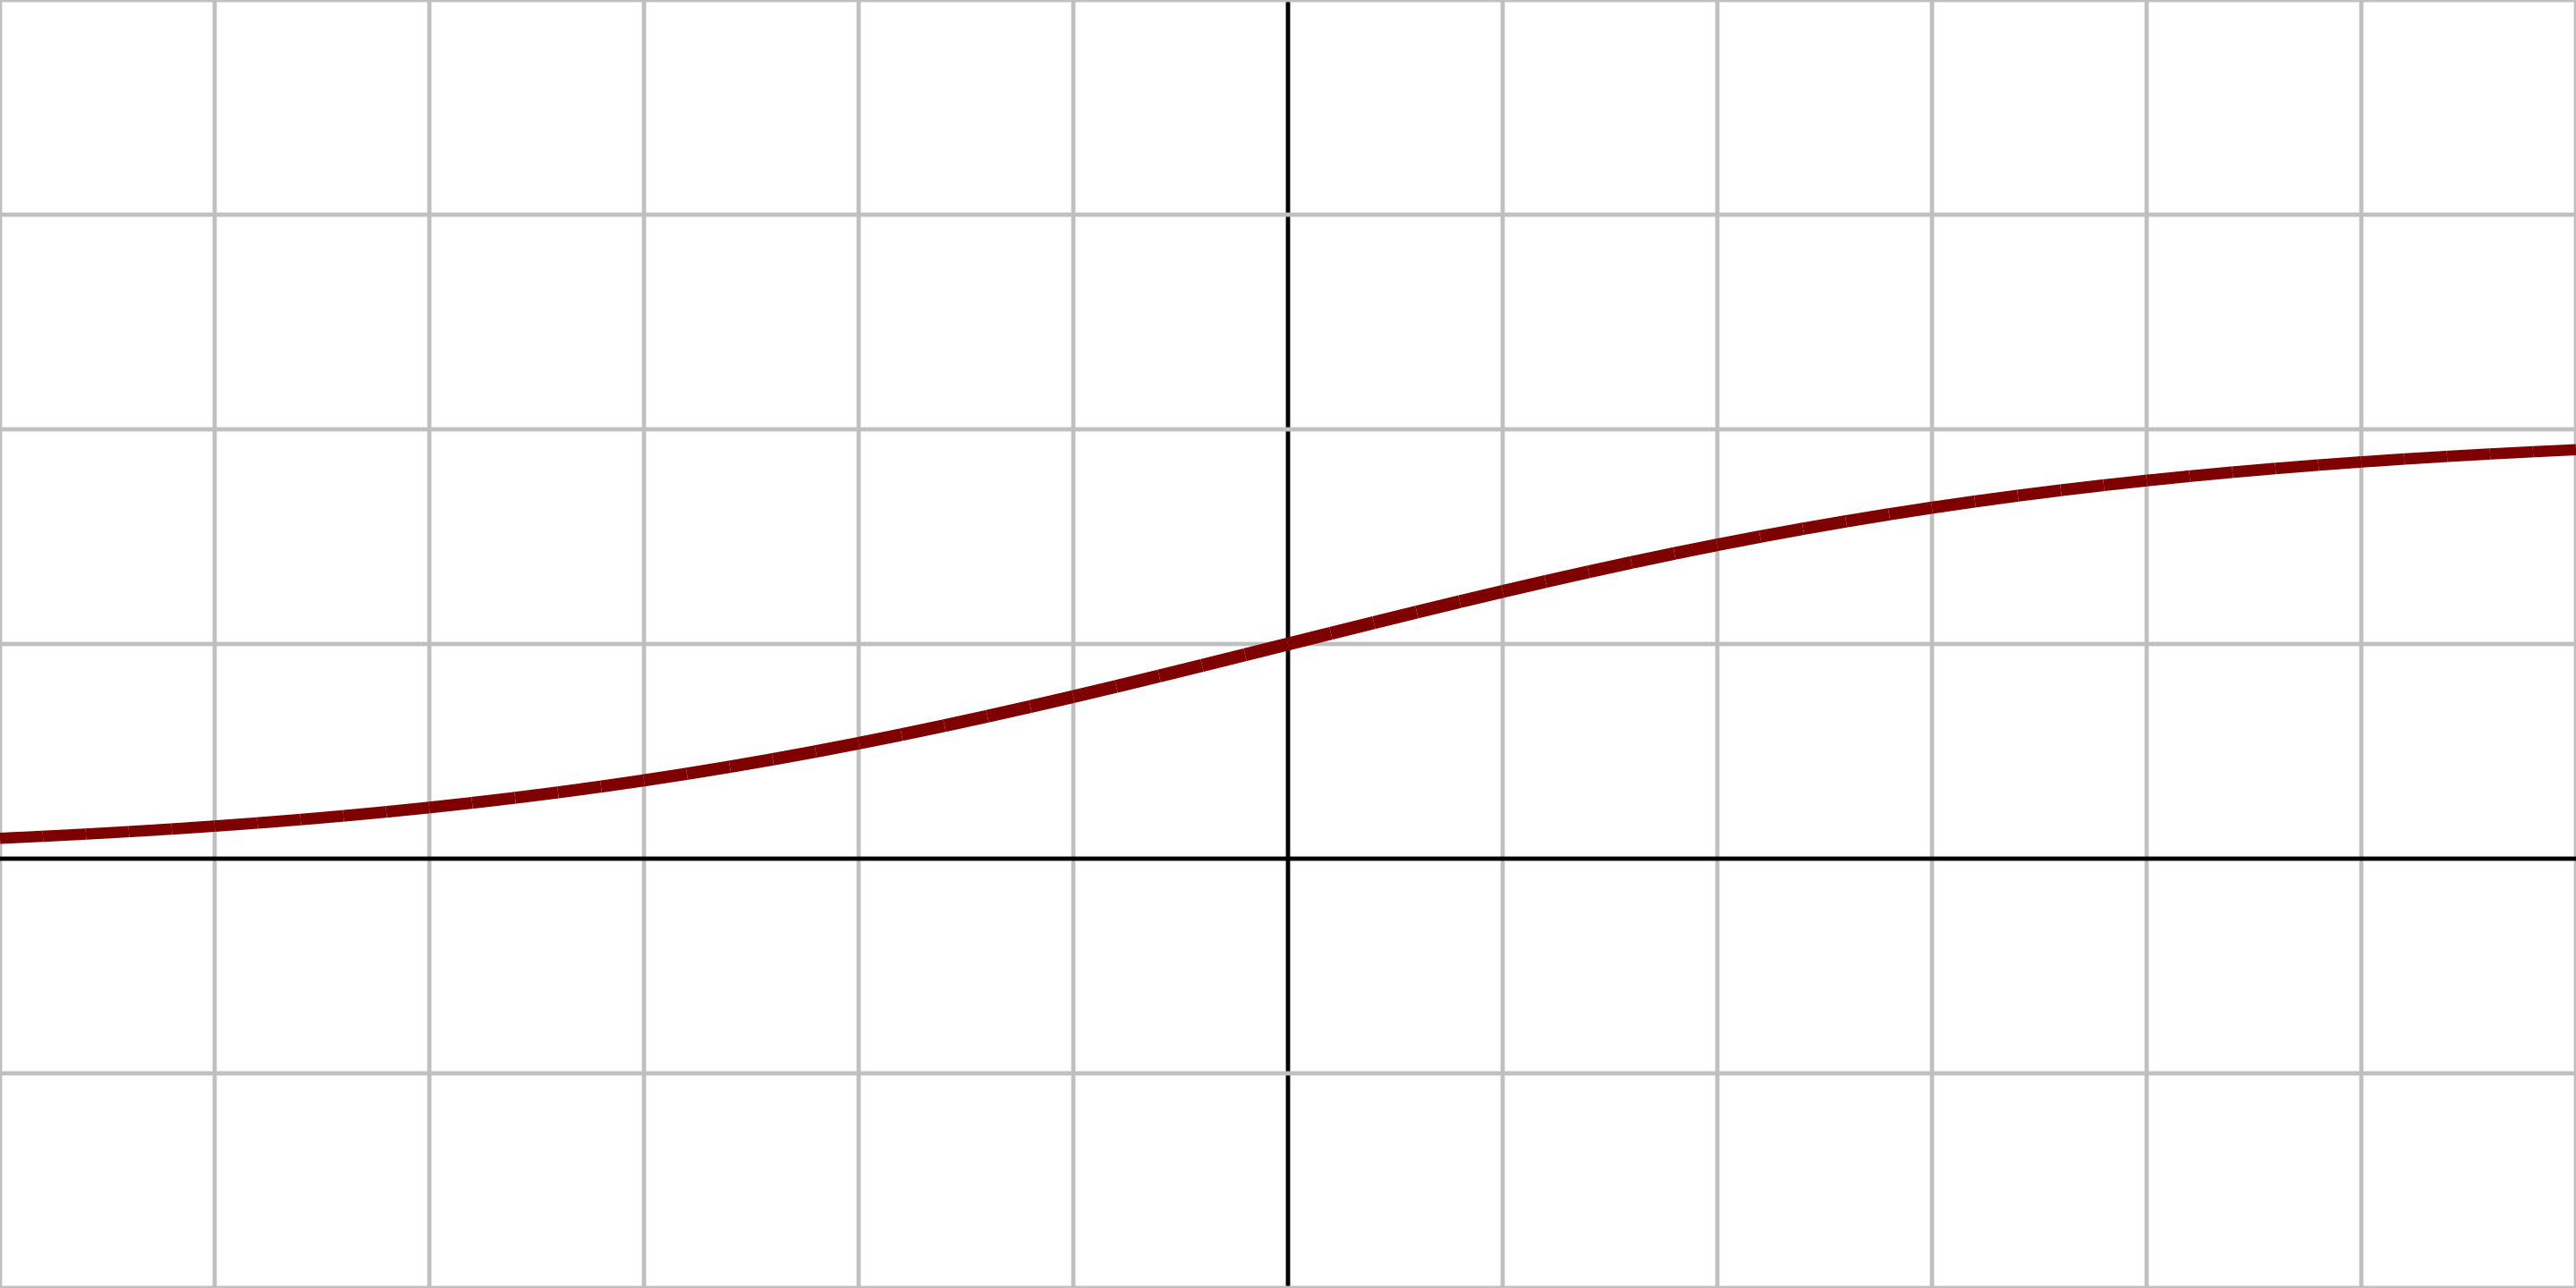
\includegraphics[width=1.8in]{images/activation_sigmoid.png}
        \label{fig:third_sub}
    }
    \caption{Activation functions \cite{activationfunction}}
    \label{activation_funtions}
\end{figure}

In multi-class classification problems, the output layer will have one neuron per class. The categories may or may not be mutually exclusive and a common way to pick the best prediction is to choose the one with the highest probability when using for example a sigmoid function. As neurons in the last hidden layer are not interconnected these probabilities are independent and need to be normalized such that their sum equals to 1. A simply function such as \textit{softmax} divides each probability by the total sum. When categories are non exclusive, a probability threshold for each output neuron such as 0.5 can be used to pick the final outcomes.

The ANN can be trained using an existing dataset of examples to make future predictions and the weights of each neuron are adjusted depending on the performance of the prediction vs the actual value. Equations such as the quadratic cost function (see eq \ref{cost_function}) or cross entropy are commonly used to make this measurement for both binary or multi-class classification. The equation provides a positive measurement of the distance from the real value. By defining \( a^L  \) as the activation function applied on \( {x_{i}} {w_{i}} \), at the last layer, the cost function takes into account a large amount of information as vectors: the weights, biases, activation function and true outcome across a number of predictions called the batch size.

\begin{eqnarray}
\label{cost_function}
  C = \frac{1}{2n} \sum_x \|y(x)-a^L(x)\|^2
\end{eqnarray}

To find the correct values for the weights and biases,  the cost function needs to be minimal. By plotting a simple version of this exponential cost function against the weight of one neuron (see fig \ref{fig:costfuntiongraph}), one could theoretically simply calculate the derivative for 0, but in reality the complexity is directly proportional to the number of neurons and will have many local minimum values making such computations infeasible.

\begin{figure}[h!]
\centering
  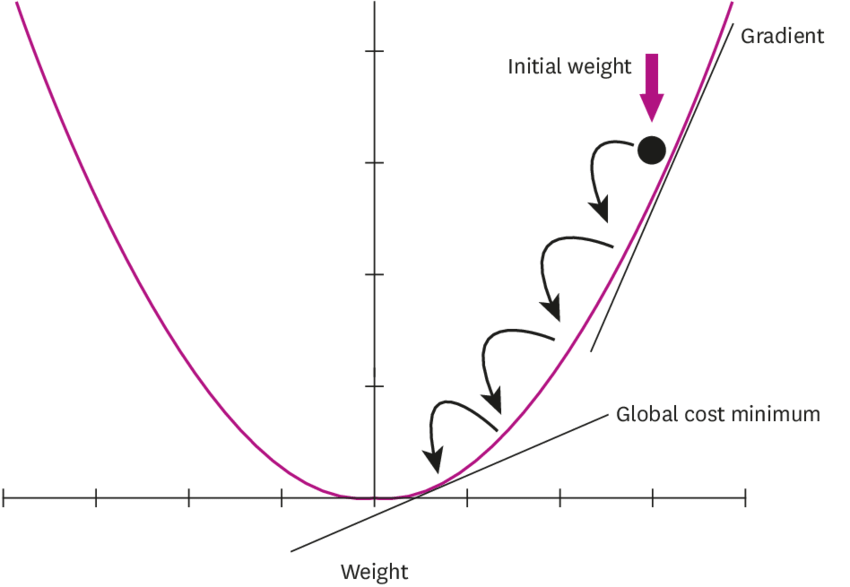
\includegraphics[scale=0.2]{images/A-graph-of-a-cost-function-modified-from.png}
  \caption{Simple cost function graph\cite{costfuntion}}
  \label{fig:costfuntiongraph}
\end{figure}

Instead, the slope can be calculated and moved downwards to find the minimum value that optimises \textit{w}, known as gradient descent. After running  a fraction or the entire dataset also known as the batch size, weights can be adjusted based on minimising the slope.  Large step sizes may overshoot the minimum while small ones will take a long time to converge. Thus, a  good approach is to adapt this learning rate and Adam\cite{kingma2014adam} is one of the best performing algorithms.

When running on the entire batch size however, the updates happen less frequently and a local minimum is more likely to be chosen instead of the global one. An alternative is to optimize weights after each input in the training data, known as stochastic gradient descent. Due to the increased update frequency, this is more likely to find a global  minimum, but is dependent on the order of the rows in the training set and is not deterministic when data is picked randomly. Finding the global minimum has many other challenges depending on the dataset, such as very big slopes or many small ones. Trusk 2015 \cite{trask} provides possible solution to these issues.

Backpropagation uses the cost function to apply changes on the weights and biases of each neuron in every layer. Taking a multi-class classification problem, such as labeling dogs, cats, and fish, the aim is to make adjustments starting from the output layer and propagating these back to the first hidden layer. If the training example has a true value of a cat and the output of the activation function has a high probability for dog, then the aim is to decrease \( a^L(x) \) for the dog label and increase the the weight for cat label using the cost function. The in depth mathematical details of the algorithm are beyond the scope of this project but the main equations including formal proofs are discussed by Nielsen 2018 \cite{nielsenneural} in chapter 2.

\section{Exploratory work}
\subsection{Building an ANN}
\subsection{Choosing a Dataset}
Kaggle\cite{kaggle} in a popular online platform for data scientists to share knowledge: this includes uploading real datasets and making them available for public use. Each dataset is open to a discussion thread and possible sample solution are discussed for different types of classification, including deep learning algorithms. Many top machine learning experts who work in the industry or academia will take part in competitions and their solutions are made public. This makes such datasets an excellent choice for the purpose of this project as a simple ANN implementation can be assessed against other solutions which arguably would end up powering real consumer products.

The Stroke dataset\cite{strokedataset} contains lifestyle and medical data about patients, some of which suffered a stroke. This is an anonymous dataset the was first published be McKinsey as part of an online Hackathon on Healthcare although the source of this information cannot be verified online. The dataset has no personal identifiable information. The 14 columns contain attributes such as gender, age, hypertension, heart disease, smoking status, or the work type of a patient. More importantly, it also specifies if a patient had a stroke which allows for classifier to be trained and make future predictions.

\subsection{Exploratory Data Analysis}
When building predictive models, a crucial part is understanding the data before building a predictive model. For example, what columns are significant in predicting a stroke? Can we derive insights based on correlations? Can some information be discarded or can missing data be filled? 

\begin{figure}
\centering
\begin{minipage}[t]{.4\textwidth}
  \centering
  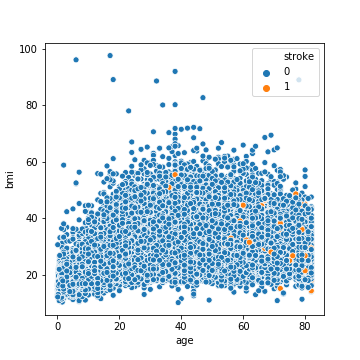
\includegraphics[width=\textwidth]{images/building_ann/age_bmi_scatterplot.png}
  \captionof{figure}{Age vs body mass index}
  \label{fig:age_bmi_scatterplot}
\end{minipage}
\begin{minipage}[t]{.5\textwidth}
  \centering
  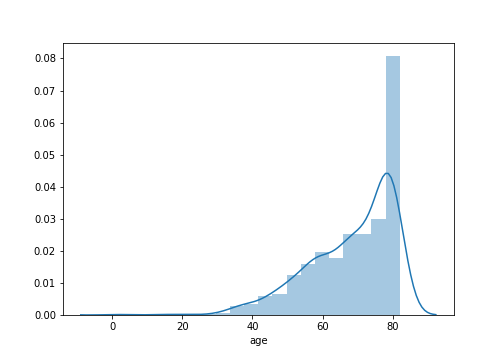
\includegraphics[width=\textwidth]{images/building_ann/stroke_age_distplot.png}
  \captionof{figure}{Age distribution of patients who suffered a stroke}
  \label{fig:age_of_stroke_patients}
\end{minipage}
\end{figure}

The stroke dataset contains 43400 entries of which only 783 (1.8\%) are patients who suffered a stroke. Intuitively, we can assume that strokes will occur more often in adults and elderly (see fig \ref{fig:age_of_stroke_patients}). A heat-map using a balanced subset (equal numbers of stroke and non-stroke patient) of the available data shows correlations among all the data columns ( fig \ref{fig:heatmap}). Missed or less intuitive correlations for a non medically trained viewer become clearer. 

For example, it is expected that age is highly correlated with a person's lifestyle choices and health such as being married, work type, having a heart disease or hypertension. It may not be immediately obvious that heart diseases and strokes follow an almost identical distribution with a higher likelihood at older ages (fig \ref{fig:age_of_stroke_patients})). Hypertension starts at earlier ages and may be a key indicator for later strokes, both having a high correlation. Another less clear correlation is the age vs the body mass index (bmi): fig \ref{fig:age_bmi_scatterplot} shows how the bmi is increasing from childhood through to adulthood and decreasing again for elderly people. Interestingly, the bmi is also correlated with the work type - this could likely be explained by the fact that those who work are also more active.

\begin{figure}[h!]
\centering
  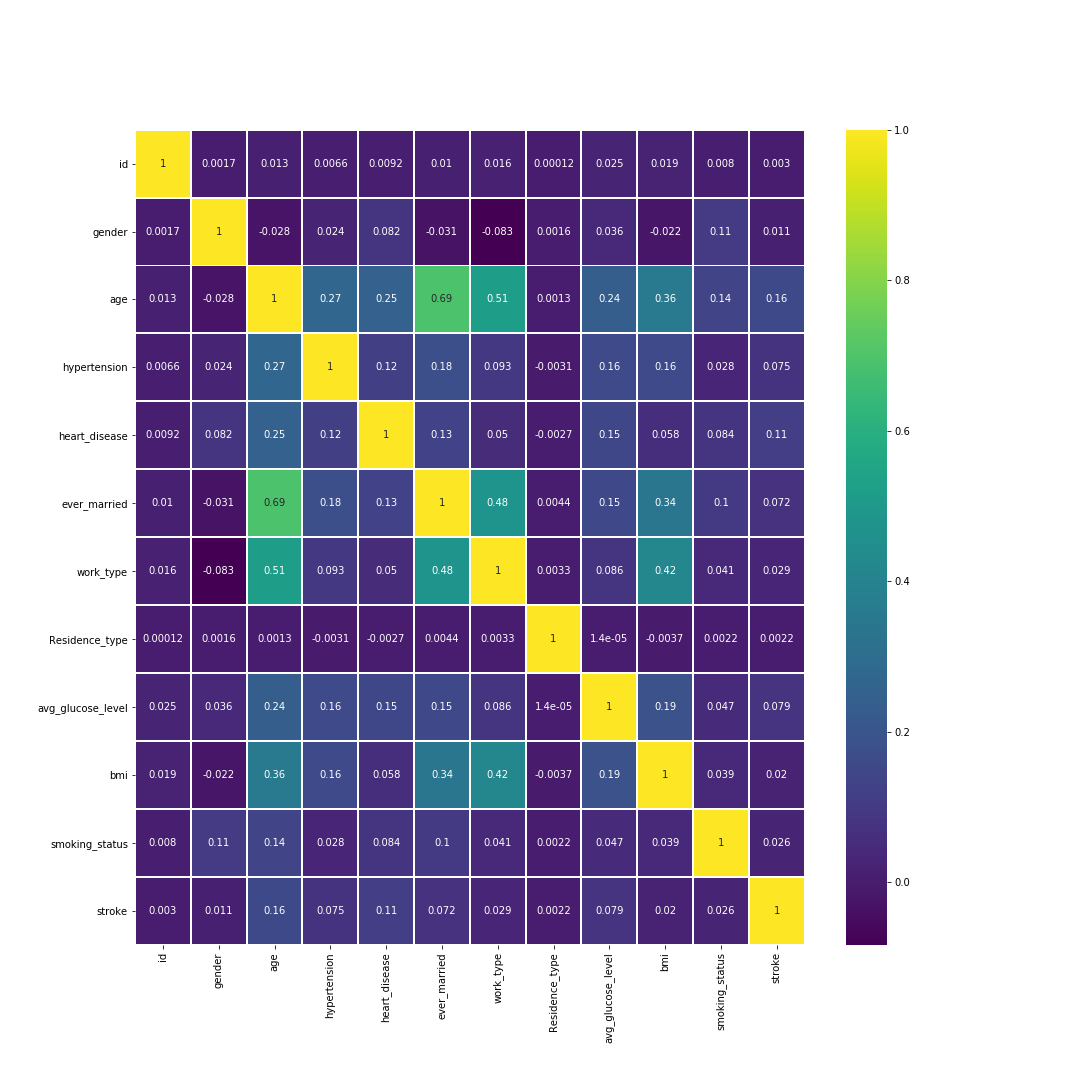
\includegraphics[width=.73\textwidth]{images/building_ann/heatmap.png}
  \caption{Correlations among all data columns using a balanced subset - smoking status is mapped to binary values}
  \label{fig:heatmap}
\end{figure}

Surprisingly, a strong correlation is seen among smoking status and gender (fig \ref{fig:gender_smoking_percentage}) than among  smoking vs strokes or hypertension. There are more males who smoke or formerly smoked than females. The number of females who never smoked is also significantly higher. Only 1.7\% of those who never smoked suffered a stroke, only slightly better than 2\% of those who regularly smoke. Unexpectedly, the highest rate of strokes is for former smokers at 3\%.

\begin{figure}[h!]
\centering
  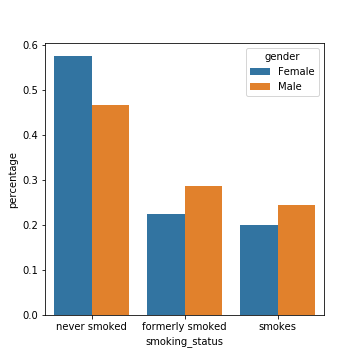
\includegraphics[width=.4\textwidth]{images/building_ann/gender_smoking_percentage.png}
  \caption{Percentage of male/female smokers}
  \label{fig:gender_smoking_percentage}
\end{figure}

\subsection{Categorical and Missing Data}
The correlations and insights derived from the previous section allow us to fill in missing data in a manner that is consistent with the dataset's features. Two columns, the \textit{bmi} and \textit{smoking status} are missing information.

There are 1462 (3.3\%) rows missing the bmi value. To ensure the dataset has no \textit{nan} values, we could simply delete these rows or replace the missing bmi with an average over the entire dataset. However, the strong correlations with age and work type allow us to be more precise: replacing the bmi with the average bmi for that age group would produce a larger distribution, but the bmi has a significantly stronger correlation (0.42) with the work type, which in turn will distribute bmi average values over five types of work. Averaging the bmi of each work type to replace missing bmi is the better choice.

The smoking column is missing in 30\% of the data. Surprisingly, this is not strongly correlated with other attributes, and has a particularly low correlation with the stroke column. A reasonable approach could be to delete the column entirely, but in a realistic scenario, stakeholders would loose confidence if they learned that smoking information has been dropped in a stroke prediction product. As such, we can fill this information using an empirical approach: if the work type is children or age is less than 18, we set this values to\textit{ never smoked}. Otherwise, we can make use of the fact that males are significantly heavier smokers and thus decide the status based on gender.

The least significant column in the dataset is the id of patients. This is a numerical value that replace personal identifiable data. This has no correlations with any attributes and should be dropped.

Categorical data needs to be mapped to numerical values for  an ANN to work. One hot encoding is used to avoid wrongly increasing the importance of a category based on it numerical mapping. For example, the column residence type will translate to columns \textit{urban} and \textit{rural} with values of 0 or 1 only. As this is duplicating the data, only one column is need and the other is dropped. For attributes with more categories, columns are created for each value  with mappings of 0 or 1. This approach ensures that no categorical value has a higher rank than others.

By creating these mapping to numerical values, the ANN will need more neurons and more processing resources. Such mappings are usually evenly distributed, but in the case of gender which has three categories (Male, Female, Other) , only 11 entries are labelled as Other out of 43400 rows. One hot encoding would add unnecessary overhead on the dataset and a good approach would be to merge such values in one of the other categories. In this case however, the eleven rows can be dropped. Finally, the number of columns after the data translation increased from 11 to 15 columns.

\subsection{Architecture of the ANN with Keras}

Keras\cite{keras} is the official api library for implementing high-level ANNs in Python using tensorflow (2.0). Hidden and output layers can be easily added with parameters such as the number of neurons or activation function to be used. A model can be trained using a large number of parameters that abstract away from the granular implementation details that would otherwise require an in depth understanding of complex mathematical formulas.

The first step is to split the dataset into a training and test set. We use 80\% to train and 20\% to test. The validation data will only be used to measure the performance and not for any training purposes during backpropagation. The data is then sclaed and normalized using the \textit{std} and \textit{min/max} values of the dataset.

The number of epochs is set to 200 with an early stopping callback to avoid over fitting after the valuation loss stops improving. Given this is an imbalanced dataset, the batch size is set to 2048 to ensure the model trains on enough rows from the minority class. The loss function is binary cross entropy with Adam as the optimizer.

On the first training attempt of the model, this achieved a 98\% accuracy. However, this metric is misleading due to the fact that the dataset is highly imbalanced. The precision for class 0 (no stroke) is nearly 99\% while 0 for the minority class 1 (suffered a stroke). The algorithm learns to always predict 0 regardless of the input. This is a common problem for Deep Learning. There are several approaches worth discussing to overcome this.

One solution is to attach weights to each class\cite{cost_sensitive}\cite{WangS}. Thus, the ANN becomes sensitive to the importance of the class: the cost function is punishing the network proportionally higher when it miscalssfies a row from the under-represented class.

The networks significantly improves when the weights are set proportionally to the class distributions \{class 0:0.51 and class 1:27.71\}. Training is stopped early after 32 epochs (fig:\ref{fig:val_loss_weighted}).  The classification report in figure   \ref{fig:weighted_ann} show how label 1 now has an 83\% recall score (TP/(TP +FN)) but only 4\% precision (TP/(TP + FP)). If this was a real medical test, it would correctly identify most of those patients who have a stroke, but would also wrongly misdiagnose 1/3 of healthy patients.


\begin{figure}
    \centering
    \subfigure
    {
    \centering
        \begin{tabular}{lrrrr}
\toprule
{} &  precision &    recall &  f1-score &       support \\
\midrule
0            &   0.994888 &  0.761424 &  0.862639 &  12780.000000 \\
1            &   0.058660 &  0.791667 &  0.109227 &    240.000000 \\
accuracy     &   0.761982 &  0.761982 &  0.761982 &      0.761982 \\
macro avg    &   0.526774 &  0.776545 &  0.485933 &  13020.000000 \\
weighted avg &   0.977630 &  0.761982 &  0.848751 &  13020.000000 \\
\bottomrule
\end{tabular}

        \label{fig:first_sub}
        \centering
    }
    \subfigure{
    \centering
        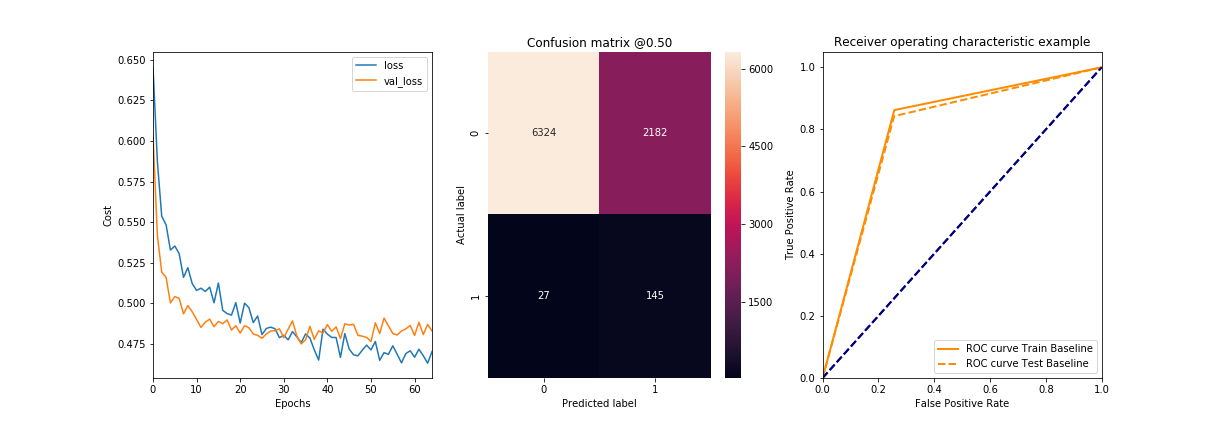
\includegraphics[width=7in]{images/building_ann/weighted.png}
        \label{fig:second_sub}
        
    }
    \caption{Weighted network}
    \label{fig:weighted_ann}
\end{figure}
   
\begin{figure}
    \centering
    \subfigure
    {
    \centering
        \begin{tabular}{lrrrr}
\toprule
{} &  precision &    recall &  f1-score &       support \\
\midrule
0            &   0.994888 &  0.761424 &  0.862639 &  12780.000000 \\
1            &   0.058660 &  0.791667 &  0.109227 &    240.000000 \\
accuracy     &   0.761982 &  0.761982 &  0.761982 &      0.761982 \\
macro avg    &   0.526774 &  0.776545 &  0.485933 &  13020.000000 \\
weighted avg &   0.977630 &  0.761982 &  0.848751 &  13020.000000 \\
\bottomrule
\end{tabular}

        \label{fig:first_sub}
        \centering
    }
    \subfigure{
    \centering
        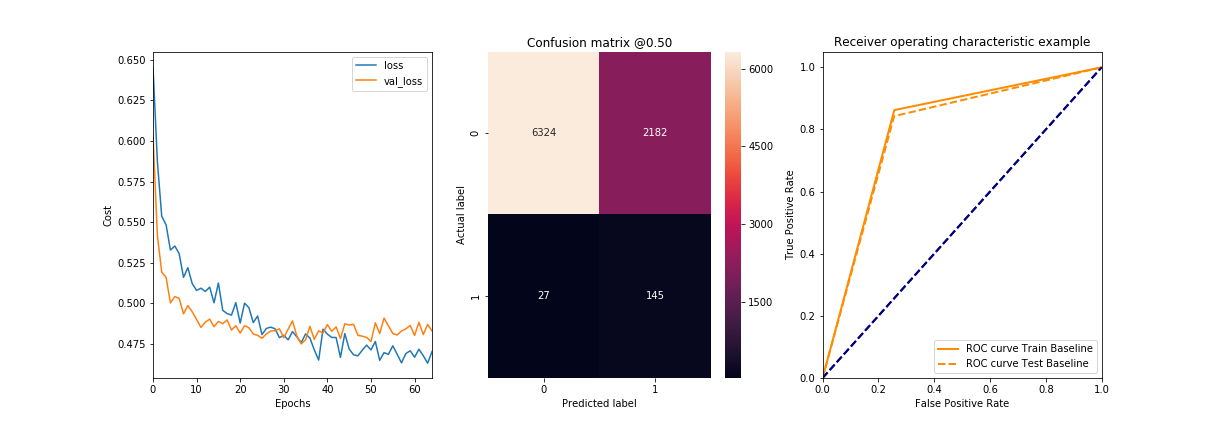
\includegraphics[width=7in]{images/building_ann/weighted.png}
        \label{fig:second_sub}
        
    }
    \caption{Weighted network}
    \label{fig:weighted_ann}
\end{figure}
   
\newpage
\footnotesize

\bibliographystyle{unsrt}
\bibliography{template}

\clearpage


\end{document}
